% These plots represent the accuracy score difference between the results obtained from the reproduction
% study and those reported in the original paper i.e. (repro_result - original_result) = points on the plot 

\begin{figure}[ht]
\centering
\usepgfplotslibrary{groupplots}
\usetikzlibrary{positioning}

\pgfplotsset{every axis title/.append style={at={(0.9,0.7)}, fill=white}}

% define name and style for each model being plotted
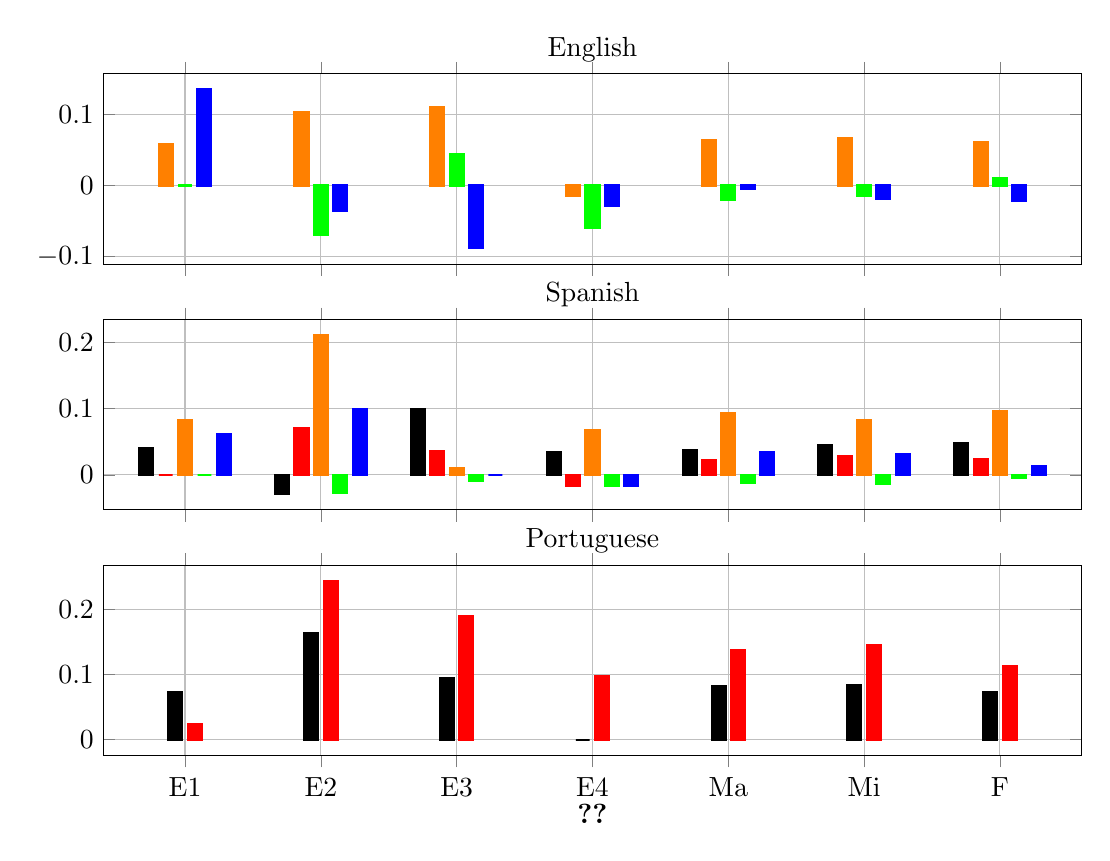
\begin{tikzpicture}[
    skipsent/.style={bar width=5pt, orange,fill=orange, thick},
    skipwv/.style={bar width=5pt, green,fill=green, thick},
    skipsyn3/.style={bar width=5pt, blue,fill=blue, thick},
    bertsent/.style={bar width=5pt, black,fill=black, thick},
    bertadd/.style={bar width=5pt, red,fill=red, thick}
]
\begin{groupplot}[
    group style={
        group name=results,
        group size=1 by 3,
        xlabels at=edge bottom,
        xticklabels at=edge bottom,
        % sets the space between the plots
        vertical sep=20pt
    },
    height=4cm,
    width=14cm,
    symbolic x coords={E1, E2, E3, E4, Ma, Mi, F},
    xtick={E1, E2, E3, E4, Ma, Mi, F},
    grid,
    ybar,
]

% ENGLISH RESULTS
\nextgroupplot
    \addplot[skipsent, ybar]
        % English fastText skip. sent: difference between Sent repro. and Sent orig. results
        coordinates {(E1, 0.058) (E2, 0.103) (E3, 0.11) (E4, -0.015)
                    (Ma, 0.064) (Mi, 0.067) (F, 0.061)};
    \addplot[skipwv, ybar]
        % English fastText skip. WV: difference between WV repro. and WV orig. results
        coordinates {(E1, 0.0) (E2, -0.069) (E3, 0.044) (E4, -0.059)
                    (Ma, -0.02) (Mi, -0.015) (F, 0.01)};
    \addplot[skipsyn3, ybar]
        % English fastText skip. Syn3: difference between Syn3 repro. and Syn3 orig. results
        coordinates {(E1, 0.135) (E2, -0.035) (E3, -0.088) (E4, -0.029)
                    (Ma, -0.004) (Mi, -0.019) (F, -0.021)};

% SPANISH RESULTS
\nextgroupplot[legend to name={CommonLegend},legend style={legend columns=5}]
    \addplot[bertsent]
        % Spanish BERT sent: difference between Sent repro. and Sent orig. results
        coordinates {(E1, 0.041) (E2, -0.029) (E3, 0.1) (E4, 0.034)
                    (Ma, 0.037) (Mi, 0.045) (F, 0.048)};
        \addlegendentry{BERT sent}

    \addplot[bertadd]
        % Spanish BERT add: difference between Add repro. and Add orig. results
        coordinates {(E1, 0.0) (E2, 0.071) (E3, 0.036) (E4, -0.017)
                    (Ma, 0.022) (Mi, 0.028) (F, 0.024)};
        \addlegendentry{BERT add}

    \addplot[skipsent]
        % Spanish fastText skip. sent: difference between Sent repro. and Sent orig. results
        coordinates {(E1, 0.082) (E2, 0.211) (E3, 0.01) (E4, 0.068)
                    (Ma, 0.093) (Mi, 0.083) (F, 0.097)};
        \addlegendentry{skip sent}
    
    \addplot[skipwv]
        % Spanish fastText skip. WV: difference between WV repro. and WV orig. results
        coordinates {(E1, 0.0) (E2, -0.028) (E3, -0.009) (E4, -0.017)
                    (Ma, -0.013) (Mi, -0.014) (F, -0.005)};
        \addlegendentry{skip wv}

    \addplot[skipsyn3]
        % Spanish fastText skip. Syn3: difference between Syn(3) repro. and Syn(3) orig. results
        coordinates {(E1, 0.062) (E2, 0.099) (E3, 0.0) (E4, -0.017)
                    (Ma, 0.035) (Mi, 0.031) (F, 0.013)};
        \addlegendentry{skip syn3}

% PORTUGUESE RESULTS
\nextgroupplot
    \addplot[bertsent]
        % Portuguese BERT sent: difference between Sent repro. and Sent orig. results
        coordinates {(E1, 0.073) (E2, 0.163) (E3, 0.095) (E4, 0.0)
                    (Ma, 0.082) (Mi, 0.083) (F, 0.073)};
    \addplot[bertadd]
        % Portuguese BERT add: difference between Add repro. and Add orig. results
        coordinates {(E1, 0.024) (E2, 0.243) (E3, 0.19) (E4, 0.097)
                    (Ma, 0.138) (Mi, 0.145) (F, 0.112)};

\end{groupplot}

% place title above each plot
\node[above = 0.03cm of results c1r1.north] {English};
\node[above = 0.03cm of results c1r2.north] {Spanish};
\node[above = 0.03cm of results c1r3.north] {Portuguese};

% place legend below last plot
\node[below = 0.5cm of results c1r3.south] {\ref*{CommonLegend}};

\end{tikzpicture}

\caption{\label{fig:acc-diff}Difference between our accuracy scores and those reported in the original paper computed across the four experiments, as well as for the macro (Ma), micro (Mi) and full (F) accuracy. For each language, only the models for which a discrepancy is observed are considered.
}

\end{figure}
